\documentclass[rnd]{mas_proposal}
% \documentclass[thesis]{mas_proposal}

\usepackage[utf8]{inputenc}
\usepackage{amsmath}
\usepackage{amsfonts}
\usepackage{amssymb}
\usepackage{graphicx}

\title{Project Proposal Title}
\author{FirstName LastName}
\supervisors{First Supervisor\\Second Supervisor \\ Third Supervisor}

% \thirdpartylogo{path/to/your/image}

\begin{document}

\maketitle

\pagestyle{plain}

\chapter{Introduction}
\begin{itemize}
    \item An introduction to the general topic you are covering.
    \item Why is it important?
\end{itemize}

\section{Problem Statement}
\begin{itemize}
    \item What are you going to solve?
    \item How are you evaluating?
\end{itemize}


\chapter{Related Work}
\begin{itemize}
    \item What have other people done?
    \item Why is it not sufficient?
\end{itemize}

\section{Section 1}
\section{Section 2}



\chapter{Project Plan}

\section{Work Packages}
The bare minimum will include the following packages:
\begin{enumerate}
    \item[WP1] Literature Search
    \item[WP2] Experiments
    \item[WP3] Project Report
\end{enumerate}
Keep in mind that depending on your project, you will probably need to add work packages that are more suited to your projects.

\section{Milestones}
\begin{enumerate}
    \item[M1] Literature search
    \item[M2] Experimental setup
    \item[M3] Experimental Analysis
    \item[M4] Report submission
\end{enumerate}

\section{Project Schedule}
Include a gantt chart here. It doesn't have to be detailed, but it should include the milestones you mentioned above.
Make sure to include the writing of your report throughout the whole project, not just at the end.

\begin{figure}[h!]
    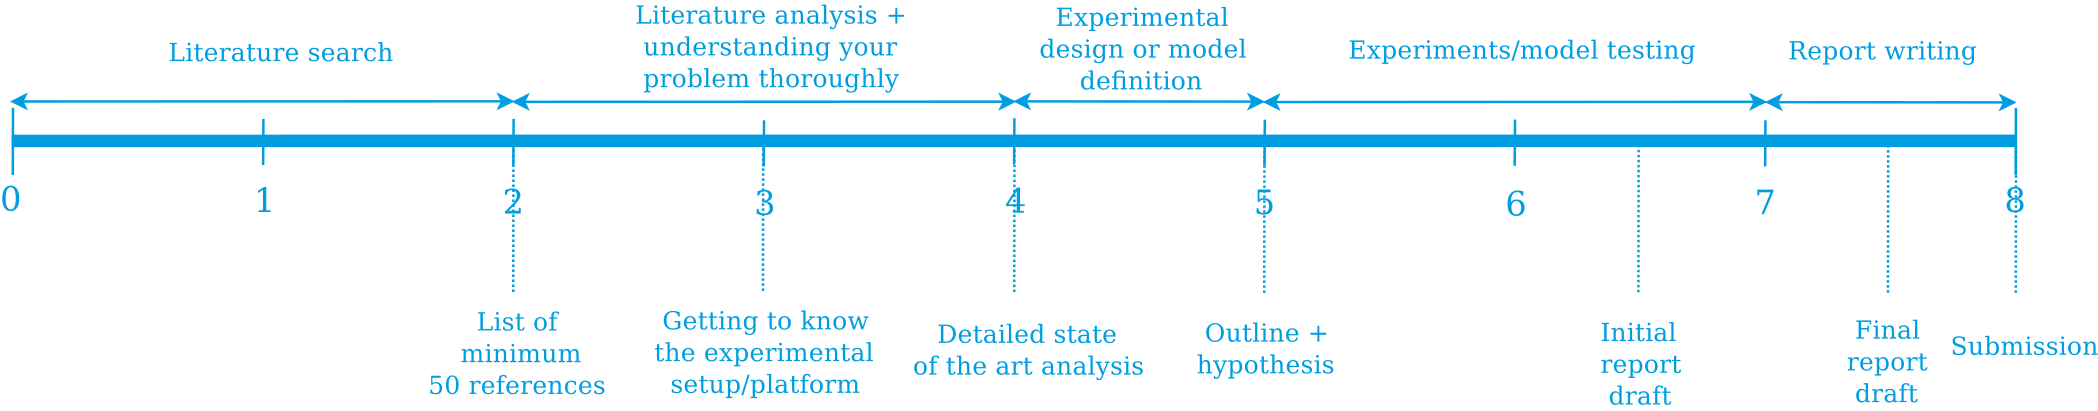
\includegraphics[width=\textwidth]{rnd_deliverable_timeline}
    \caption{}
    \label{}
\end{figure}

\section{Deliverables}
\subsection{Minimum Viable}

\begin{itemize}
    \item Survey
    \item Analysis of state of the art
    \item Simple simulated use case
    \item Demo on youBot or Jenny
\end{itemize}

\subsection{Expected}
\begin{itemize}
    \item Comparation of approaches in the robot
\end{itemize}

\subsection{Desired}
\begin{itemize}
    \item Integration to scenario
\end{itemize}


\nocite{*}

\bibliographystyle{plainnat} % Use the plainnat bibliography style
\bibliography{bibliography.bib} % Use the bibliography.bib file as the source of references




\end{document}
